%%%%%% 注意: 使用XeLaTeX编译
\documentclass[a4paper, 11pt]{article}
\usepackage{amsmath} %数学函数
%\usepackage{ctex} %中文支持
%中文包
\usepackage[UTF8]{ctex}
\usepackage{geometry}  %文档边距
%\usepackage{c} %画图
\usepackage{tikz}
\usepackage{multicol} %分栏
\usepackage{verbatim}
%\usetikzlibrary{arrows,automata}
\usetikzlibrary{automata, positioning} %自动机
\usepackage{pgf}
\usetikzlibrary{arrows, decorations.pathmorphing, backgrounds, positioning, fit, petri, automata}
\definecolor{yellow1}{rgb}{1,0.8,0.2}
\geometry{left=2.0cm,right=2.0cm,top=2.5cm,bottom=2.5cm} 
\begin{document}
\title{Homework2}
\author{Wang Taiwu, NO. 18S151560}
\maketitle

1.29. 使用泵引理证明下述语言不是正则的.\\
\textbf{1.29. Using the pump principle to prove that the language is not regular.}
\\ (b). $A_2=\{www|w\in \{a, b\}*\}$
\\ \textbf{Proof:}
\\ \indent Using the proof of contradiction. Assuming $A_2$ is regular. p is the length given by the pump principle. Let s be a string $a^pba^pba^pb$. Because s is a member of the $A_2$, and the lenght of s is greater than p, so the pump lemma to ensure that s can be divided into 3 sections, s = xyz. Considering the third condition of the pump lemma, which is said | xy | < p, so y only containes a. Because $A_2=\{www|w\in\{a, b\}\}$ xyyz is not a member of $A_2$. There was a contradiction here. That is to say, the language $A_2$ is not regular.
\\

\textbf{1.36. Let $B_n$=\{$a^k$ | k is an integer multiple of n\}. Proof: For each n $\geq$ 1, the language $B_n$ is regular.  }
 \\ \textbf{Proof:}
 \\ \indent For any $n \geq 1$, if $B_n$ can be identified by a DFA, then $B_n$ is regular. 
 \begin{multicols}{2}
 \begin{center}
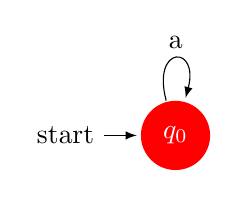
\begin{tikzpicture}[>=latex, shorten >=1pt,node distance=0.75in, on grid, auto]

\tikzstyle{every state}=[fill=red,draw=none,text=white]

% Vertices of automaton
\node[state, initial, accepting] (q0) {$q_0$};
%\node[state, accepting] (q1) [right=of q0] {$q_1$};
% Edges of automaton
\path[->] 
(q0) edge [loop above] node {a} (q1);
%(q1) edge  [bend left] node [swap] {$\varepsilon$}(q0);
\end{tikzpicture}
\\ Figure 1: DFA when n is 1.
 \end{center}
 
 \begin{center}
 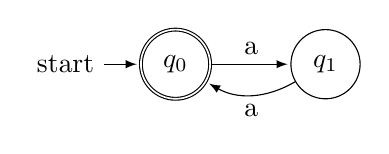
\begin{tikzpicture}[>=latex, shorten >=1pt,node distance=0.75in, on grid, auto]
 
% Vertices of automaton
\node[state, initial, accepting] (q0) {$q_0$};
\node[state](q1) [right=of q0] {$q_1$};
% \node[state, accepting] (q2) [right=of q1] {$q_2$};
% Edges of automaton
\path[->] 
(q0) edge node {a} (q1)
(q1) edge [bend left] node {a} (q0);
%(q2) edge  [bend left] node [swap] {$\varepsilon$}(q0);
\end{tikzpicture}
\\ Figure 2: DFA when n is 2.
 \end{center}
 
  \begin{center}
 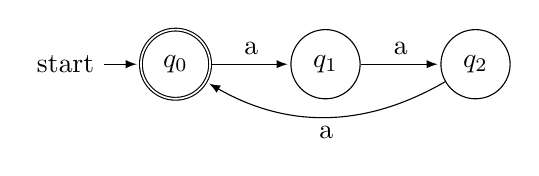
\begin{tikzpicture}[>=latex, shorten >=1pt,
node distance=0.75in, on grid, auto]
% Vertices of automaton
\node[state, initial, accepting] (q0) {$q_0$};
\node[state](q1) [right=of q0] {$q_1$};
\node[state,] (q2) [right=of q1] {$q_2$};
% Edges of automaton
\path[->] 
(q0) edge node {a} (q1)
(q1) edge node {a} (q2)
(q2) edge  [bend left] node  {a}(q0);
\end{tikzpicture}
\\ Figure 3: DFA when n is 3.
 \end{center}
 
  \begin{center}
 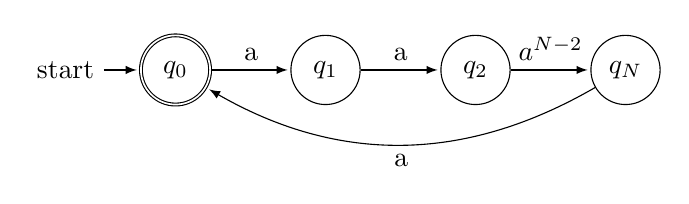
\begin{tikzpicture}[>=latex, shorten >=1pt,
node distance=0.75in, on grid, auto]
% Vertices of automaton
\node[state, initial, accepting] (q0) {$q_0$};
\node[state](q1) [right=of q0] {$q_1$};
\node[state,] (q2) [right=of q1] {$q_2$};
\node[state,] (qN) [right=of q2] {$q_N$};
% Edges of automaton
\path[->] 
(q0) edge node {a} (q1)
(q1) edge node {a} (q2)
(q2) edge node {$a^{N-2}$} (qN)
(qN) edge  [bend left] node  {a}(q0);
\end{tikzpicture}
\\ Figure 4: GNFA when n is N+1.
 \end{center}
 \end{multicols}
 From the figures above, we can see that for each $n$, we can find a DFA recognize the language $B_{n}$. So, the language $B_{n}$ is regular.
 
 
 \textbf{1.49.  Prove the following proposition:}
 \\ a. Let $B$=\{$1^{k}|y \in $ \{0, 1\}* and y contains at least k 1s, for k $\geq$1\}.
 \\ b. Let $C$=\{ $1^{k} y|y\in $\{0, 1\}* and y contains at most k 1s, for k $\geq$1\}.
 \\ \textbf{Proof:}
 \\ a. 
 \\ \indent For any $k \geq 1$, we can construct DFA as belows:
 \begin{center}
 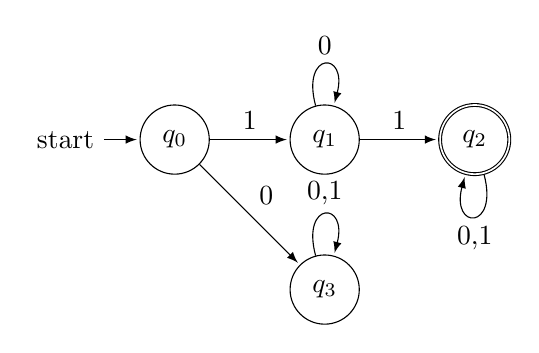
\begin{tikzpicture}[>=latex, shorten >=1pt, node distance=0.75in, on grid, auto]
% Vertices of automaton
\node[state, initial] (q0) {$q_0$};
\node[state] (q1)[right=of q0] {$q_{1}$};
\node[state, accepting](q2)[right=of q1]{$q_{2}$};
\node[state] (q3)[below= of q1]  {$q_3$};
% Edges of automaton
\path[->] 
(q0) edge node {0} (q3)
(q0) edge node{1} (q1)
(q1) edge node{1}(q2)
(q2) edge[loop below] node{0,1}(q2)
(q1) edge[loop above] node {0}(q1)
(q3) edge [loop above] node{0,1} (q3);
%(q1) edge  [bend left] node [swap] {$\varepsilon$}(q0);
\end{tikzpicture}
\\ Figure 5: DFA when k is 1.


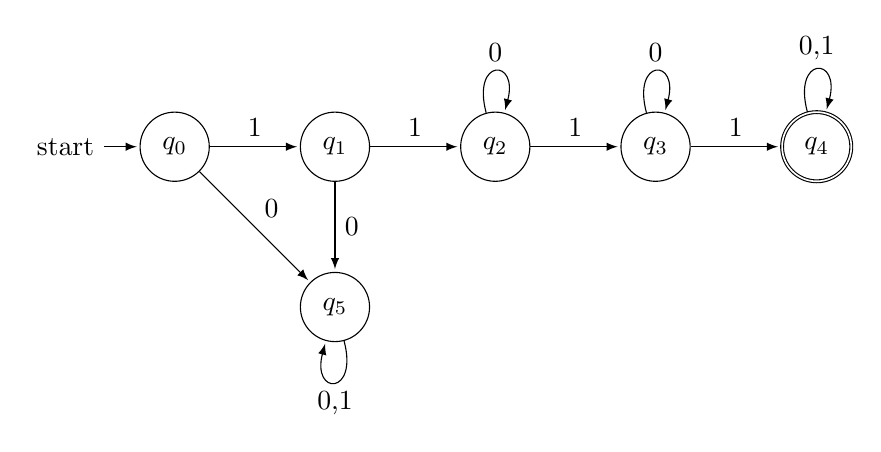
\begin{tikzpicture}[>=latex, shorten >=1pt, node distance=0.45in, auto]
% Vertices of automaton
\node[state, initial] (q0) at (1,0){$q_0$};
\node[state] (q1)[right=of q0] {$q_{1}$};
\node[state] (q2)[right=of q1] {$q_{2}$};
\node[state] (q3)[right=of q2] {$q_{3}$};
\node[state,accepting] (q4)[right=of q3] {$q_{4}$};
\node[state] (q5)[below= of q1]  {$q_5$};
% Edges of automaton
\path[->] 
(q0) edge node {0} (q5)
(q0) edge node{1} (q1)
(q1) edge node{1}(q2)
(q1) edge node{0}(q5)
(q2) edge node{1}(q3)
(q3) edge node{1}(q4)
(q5) edge[loop below] node{0,1}(q5)
(q2) edge[loop above] node {0}(q2)
(q3) edge[loop above] node {0}(q3)
(q4) edge [loop above] node{0,1} (q4);
%(q1) edge  [bend left,swap] node {$\varepsilon$}(q0);
\end{tikzpicture}
\\ Figure 6: DFA when k is 2.

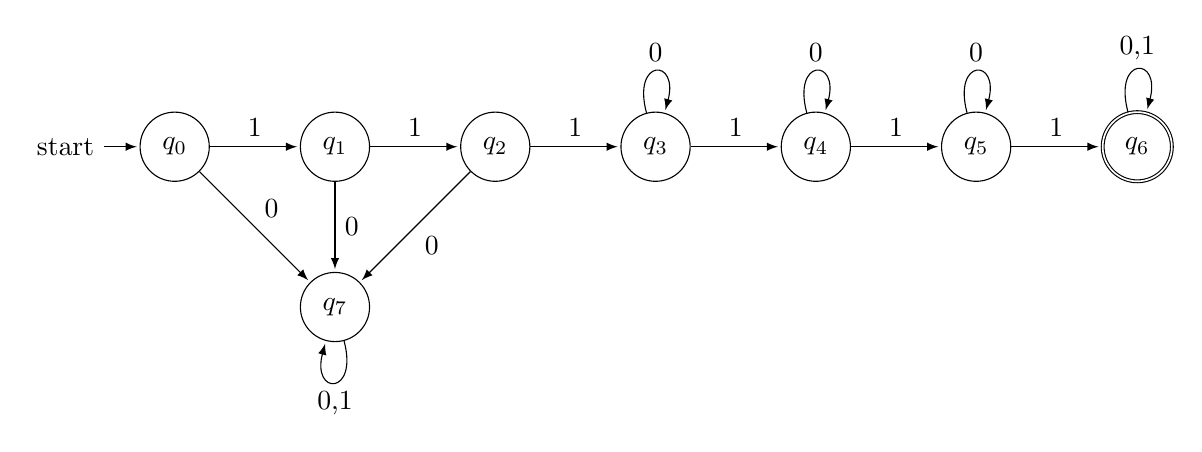
\begin{tikzpicture}[>=latex, shorten >=1pt, node distance=0.45in, auto]
% Vertices of automaton
\node[state, initial] (q0) at (1,0){$q_0$};
\node[state] (q1)[right=of q0] {$q_{1}$};
\node[state] (q2)[right=of q1] {$q_{2}$};
\node[state] (q3)[right=of q2] {$q_{3}$};
\node[state] (q4)[right=of q3] {$q_{4}$};
\node[state] (q5)[right=of q4] {$q_{5}$};
\node[state,accepting] (q6)[right=of q5] {$q_{6}$};
\node[state] (q7)[below= of q1]  {$q_7$};
% Edges of automaton
\path[->] 
(q0) edge node {0} (q7)
(q0) edge node{1} (q1)
(q1) edge node{1}(q2)
(q1) edge node{0}(q7)
(q2) edge node{1}(q3)
(q2) edge node{0}(q7)
(q3) edge node{1}(q4)
(q4) edge node{1}(q5)
(q5) edge node{1}(q6)
(q7) edge[loop below] node{0,1}(q7)
(q3) edge[loop above] node {0}(q3)
(q4) edge[loop above] node {0}(q4)
(q5) edge[loop above] node {0}(q5)
(q6) edge [loop above] node{0,1} (q6);
%(q1) edge  [bend left,swap] node {$\varepsilon$}(q0);
\end{tikzpicture}
\\ Figure 7: DFA when k is 3.

\end{center}
As shown in the figures above, for any k$\geq$1, we can construct DFA, that there are k states like state $q_{2}$ and k states like state $q_{3}$ in figure 7.
\\ b. 
\\ \indent Using proof of contradiction. Assuming $C$ is regular, p is the length given by the pump principle. Let s be a string $1^{p}01^{p}$. Because s is a member of $C$, and the length of s is grater than p, so the pump lemma to ensure that s can be divided into 3 parts, s=xyz. Considering the third condition of the pump lemma, whilch is said | xy | < p. So y only contains 1. Assume the number of 1 which y ontains is m. Then xyyz=$1^{p-m}1^{m}1^{m}01^{p}=1^{p+m}01^{p}$. Because xyyz is not a member of C. There was a contradiction here. So the assumption is not true, $C$ is not regular.

\textbf{2.10. Given an context free grammar that produces the language $A=\{a^{i}b^{j}c^{k}|i, j, k \geq 0 \ and \ i=j\  or\  j=k\}$. Is it ambiguous? why?}
\\ \textbf{Answer:}
\\ \indent We can give a CFG that can generate A as the fllowing form:
$$G=\{\{S, A, B, X, Y\},\{a, b, c, d\}, R, S\}$$
 The rules set $R$ is:
\begin{align}
S &\rightarrow XA | BY 
\\ X &\rightarrow Xa | a
\\ A &\rightarrow bAc | \varepsilon
\\ B &\rightarrow aBb | \varepsilon
\\ Y &\rightarrow Yc |c
\end{align}
\indent The context-free grammar given by me is ambiguous. Because the string abc have two different leftmost derivations.
\begin{align}
 a. \ \ S\Rightarrow XA\Rightarrow aA\Rightarrow abAc\Rightarrow abc
\\ b. \ \ S\Rightarrow BY\Rightarrow Bc\Rightarrow aBbc\Rightarrow abc
\end{align}
\\So, the context-free grammar G is ambiguous.








\iffalse
\begin{tikzpicture}[->,>=stealth',shorten >=1pt,auto,node distance=2.8cm,
                    semithick]
  \tikzstyle{every state}=[fill=yellow1,draw=none,text=black]

  \node[state]         (S) at (-6, 0)              {S};
  \node[state]         (xin1) at (-2, 3)           {X1in};
  \node[state]         (xin2) at (-2, 1)        {X2in};
  \node[state]         (xin3) at (-2, -1)       {X3in};
  \node[state]         (xin4) at (-2, -3)           {X4in};
  \node[state]         (xout1) at (0, 3)          {X1out};
  \node[state]         (xout2) at (0, 1)        {X2out};
  \node[state]         (xout3) at (0, -1)   {X3out};
  \node[state]         (xout4) at (0, -3)           {X4out};
  \node[state]         (xin5)  at (3, -2)   {X5in};
  \node[state]         (xout5) at (5, -2)   {X5out};
  \node[state]         (DC) at (7, 2)           {DC};

  \path (S) edge[bend left=26]              node {∞} (xin1)
            edge[bend left=12]              node {∞} (xin2)
            edge[bend right=12]             node {∞} (xin3)
            edge[bend right=26]             node {∞} (xin4)
        (xin1) edge  node {α=1} (xout1)
        (xin2) edge  node {α=1} (xout2)
        (xin3) edge  node {α=1} (xout3)
        (xin4) edge  node {α=1} (xout4)
        (xin5) edge  node {1} (xout5);
  \draw[->] (xout1) to[out=-30,in=150] node {β} (xin5);
  \draw[->] (xout2.east) to[out=-15,in=165] node [below] {β} (xin5);
  \draw[->] (xout3.east) to[out=0,in=180] node [below] {β} (xin5.west);
  \draw[->] (xout1) to[out=-5,in=175] node {∞} (DC);
  \draw[->] (xout5) to[out=40, in=-120] node {∞} (DC);
\end{tikzpicture}



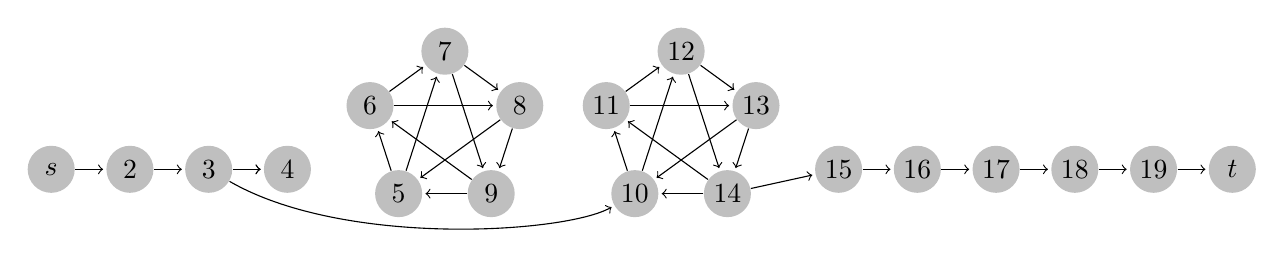
\begin{tikzpicture}[shorten >=1pt,->]
  \tikzstyle{vertex}=[circle,fill=black!25,minimum size=17pt,inner sep=0pt]

  \foreach \name/\x in {s/1, 2/2, 3/3, 4/4, 15/11, 
                        16/12, 17/13, 18/14, 19/15, t/16}
    \node[vertex] (G-\name) at (\x,0) {$\name$};

  \foreach \name/\angle/\text in {P-1/234/5, P-2/162/6, 
                                  P-3/90/7, P-4/18/8, P-5/-54/9}
    \node[vertex,xshift=6cm,yshift=.5cm] (\name) at (\angle:1cm) {$\text$};

  \foreach \name/\angle/\text in {Q-1/234/10, Q-2/162/11, 
                                  Q-3/90/12, Q-4/18/13, Q-5/-54/14}
    \node[vertex,xshift=9cm,yshift=.5cm] (\name) at (\angle:1cm) {$\text$};

  \foreach \from/\to in {s/2,2/3,3/4,3/4,15/16,16/17,17/18,18/19,19/t}
    \draw (G-\from) -- (G-\to);

  \foreach \from/\to in {1/2,2/3,3/4,4/5,5/1,1/3,2/4,3/5,4/1,5/2}
    { \draw (P-\from) -- (P-\to); \draw (Q-\from) -- (Q-\to); }

  \draw (G-3) .. controls +(-30:2cm) and +(-150:1cm) .. (Q-1);
  \draw (Q-5) -- (G-15);
\end{tikzpicture}
\fi
\end{document}
